% Options for packages loaded elsewhere
\PassOptionsToPackage{unicode}{hyperref}
\PassOptionsToPackage{hyphens}{url}
%
\documentclass[
  8pt,
  ignorenonframetext,
]{beamer}
\usepackage{pgfpages}
\setbeamertemplate{caption}[numbered]
\setbeamertemplate{caption label separator}{: }
\setbeamercolor{caption name}{fg=normal text.fg}
\beamertemplatenavigationsymbolsempty
% Prevent slide breaks in the middle of a paragraph
\widowpenalties 1 10000
\raggedbottom
\setbeamertemplate{part page}{
  \centering
  \begin{beamercolorbox}[sep=16pt,center]{part title}
    \usebeamerfont{part title}\insertpart\par
  \end{beamercolorbox}
}
\setbeamertemplate{section page}{
  \centering
  \begin{beamercolorbox}[sep=12pt,center]{part title}
    \usebeamerfont{section title}\insertsection\par
  \end{beamercolorbox}
}
\setbeamertemplate{subsection page}{
  \centering
  \begin{beamercolorbox}[sep=8pt,center]{part title}
    \usebeamerfont{subsection title}\insertsubsection\par
  \end{beamercolorbox}
}
\AtBeginPart{
  \frame{\partpage}
}
\AtBeginSection{
  \ifbibliography
  \else
    \frame{\sectionpage}
  \fi
}
\AtBeginSubsection{
  \frame{\subsectionpage}
}
\usepackage{amsmath,amssymb}
\usepackage{lmodern}
\usepackage{iftex}
\ifPDFTeX
  \usepackage[T1]{fontenc}
  \usepackage[utf8]{inputenc}
  \usepackage{textcomp} % provide euro and other symbols
\else % if luatex or xetex
  \usepackage{unicode-math}
  \defaultfontfeatures{Scale=MatchLowercase}
  \defaultfontfeatures[\rmfamily]{Ligatures=TeX,Scale=1}
\fi
% Use upquote if available, for straight quotes in verbatim environments
\IfFileExists{upquote.sty}{\usepackage{upquote}}{}
\IfFileExists{microtype.sty}{% use microtype if available
  \usepackage[]{microtype}
  \UseMicrotypeSet[protrusion]{basicmath} % disable protrusion for tt fonts
}{}
\makeatletter
\@ifundefined{KOMAClassName}{% if non-KOMA class
  \IfFileExists{parskip.sty}{%
    \usepackage{parskip}
  }{% else
    \setlength{\parindent}{0pt}
    \setlength{\parskip}{6pt plus 2pt minus 1pt}}
}{% if KOMA class
  \KOMAoptions{parskip=half}}
\makeatother
\usepackage{xcolor}
\newif\ifbibliography
\usepackage{color}
\usepackage{fancyvrb}
\newcommand{\VerbBar}{|}
\newcommand{\VERB}{\Verb[commandchars=\\\{\}]}
\DefineVerbatimEnvironment{Highlighting}{Verbatim}{commandchars=\\\{\}}
% Add ',fontsize=\small' for more characters per line
\usepackage{framed}
\definecolor{shadecolor}{RGB}{248,248,248}
\newenvironment{Shaded}{\begin{snugshade}}{\end{snugshade}}
\newcommand{\AlertTok}[1]{\textcolor[rgb]{0.94,0.16,0.16}{#1}}
\newcommand{\AnnotationTok}[1]{\textcolor[rgb]{0.56,0.35,0.01}{\textbf{\textit{#1}}}}
\newcommand{\AttributeTok}[1]{\textcolor[rgb]{0.77,0.63,0.00}{#1}}
\newcommand{\BaseNTok}[1]{\textcolor[rgb]{0.00,0.00,0.81}{#1}}
\newcommand{\BuiltInTok}[1]{#1}
\newcommand{\CharTok}[1]{\textcolor[rgb]{0.31,0.60,0.02}{#1}}
\newcommand{\CommentTok}[1]{\textcolor[rgb]{0.56,0.35,0.01}{\textit{#1}}}
\newcommand{\CommentVarTok}[1]{\textcolor[rgb]{0.56,0.35,0.01}{\textbf{\textit{#1}}}}
\newcommand{\ConstantTok}[1]{\textcolor[rgb]{0.00,0.00,0.00}{#1}}
\newcommand{\ControlFlowTok}[1]{\textcolor[rgb]{0.13,0.29,0.53}{\textbf{#1}}}
\newcommand{\DataTypeTok}[1]{\textcolor[rgb]{0.13,0.29,0.53}{#1}}
\newcommand{\DecValTok}[1]{\textcolor[rgb]{0.00,0.00,0.81}{#1}}
\newcommand{\DocumentationTok}[1]{\textcolor[rgb]{0.56,0.35,0.01}{\textbf{\textit{#1}}}}
\newcommand{\ErrorTok}[1]{\textcolor[rgb]{0.64,0.00,0.00}{\textbf{#1}}}
\newcommand{\ExtensionTok}[1]{#1}
\newcommand{\FloatTok}[1]{\textcolor[rgb]{0.00,0.00,0.81}{#1}}
\newcommand{\FunctionTok}[1]{\textcolor[rgb]{0.00,0.00,0.00}{#1}}
\newcommand{\ImportTok}[1]{#1}
\newcommand{\InformationTok}[1]{\textcolor[rgb]{0.56,0.35,0.01}{\textbf{\textit{#1}}}}
\newcommand{\KeywordTok}[1]{\textcolor[rgb]{0.13,0.29,0.53}{\textbf{#1}}}
\newcommand{\NormalTok}[1]{#1}
\newcommand{\OperatorTok}[1]{\textcolor[rgb]{0.81,0.36,0.00}{\textbf{#1}}}
\newcommand{\OtherTok}[1]{\textcolor[rgb]{0.56,0.35,0.01}{#1}}
\newcommand{\PreprocessorTok}[1]{\textcolor[rgb]{0.56,0.35,0.01}{\textit{#1}}}
\newcommand{\RegionMarkerTok}[1]{#1}
\newcommand{\SpecialCharTok}[1]{\textcolor[rgb]{0.00,0.00,0.00}{#1}}
\newcommand{\SpecialStringTok}[1]{\textcolor[rgb]{0.31,0.60,0.02}{#1}}
\newcommand{\StringTok}[1]{\textcolor[rgb]{0.31,0.60,0.02}{#1}}
\newcommand{\VariableTok}[1]{\textcolor[rgb]{0.00,0.00,0.00}{#1}}
\newcommand{\VerbatimStringTok}[1]{\textcolor[rgb]{0.31,0.60,0.02}{#1}}
\newcommand{\WarningTok}[1]{\textcolor[rgb]{0.56,0.35,0.01}{\textbf{\textit{#1}}}}
\setlength{\emergencystretch}{3em} % prevent overfull lines
\providecommand{\tightlist}{%
  \setlength{\itemsep}{0pt}\setlength{\parskip}{0pt}}
\setcounter{secnumdepth}{-\maxdimen} % remove section numbering
% type setting
% ------------------------------------------------------------------------------
\usepackage[german]{babel}     

% fonts
% ------------------------------------------------------------------------------
\usefonttheme{professionalfonts}

% slide title and horizontal line
% ------------------------------------------------------------------------------
\setbeamertemplate{frametitle}{%
    \vskip-30pt \color{black}\large%
    \begin{minipage}[b][23pt]{120mm}%
    \flushleft\insertframetitle%
    \end{minipage}%
}

\setbeamertemplate{headline}										
{
\vskip10pt\hfill\hspace{3.5mm} 										 
\vskip15pt\color{black}\rule{\textwidth}{0.4pt} 					 
}

% slide number
% ---------------------------------------------------------------
\setbeamertemplate{navigation symbols}{}
\setbeamertemplate{footline}
{
\vskip5pt
\vskip2pt
\makebox[123mm]{\hspace{7.5mm}
\hfill Allgemeines Lineares Modell - Tutorium $\vert$ 
Sean Mulready $\vert$
Folie \insertframenumber}
\vskip4pt
}

% block color scheme
% ------------------------------------------------------------------------------
% colors
\definecolor{white}{RGB}{255,255,255}
\definecolor{grey}{RGB}{205,205,205}
\definecolor{lightgrey}{RGB}{245,245,245}
\definecolor{LightBlue}{RGB}{220,220,255}
\definecolor{darkblue}{RGB}{51, 51, 153}
\definecolor{darkcyan}{RGB}{0,102,102}
\definecolor{middlecyan}{RGB}{0,153,153}
\definecolor{darkgreen}{RGB}{0,102,51}
\definecolor{plum}{RGB}{128,0,128}
\definecolor{orange}{RGB}{255,141,42}

% definitions and theorems
\setbeamercolor{block title}{fg = black, bg = grey}
\setbeamercolor{block body}{fg = black, bg = lightgrey}

% general line spacing 
% ------------------------------------------------------------------------------
\linespread{1.3}

% local line spacing
% ------------------------------------------------------------------------------
\usepackage{setspace}

% colors
% -----------------------------------------------------------------------------
\usepackage{color}

% justified text
% ------------------------------------------------------------------------------
\usepackage{ragged2e}
\usepackage{etoolbox}
\apptocmd{\frame}{}{\justifying}{}

% bullet point lists
% -----------------------------------------------------------------------------
\setbeamertemplate{itemize item}[circle]
\setbeamertemplate{itemize subitem}[circle]
\setbeamertemplate{itemize subsubitem}[circle]
\setbeamercolor{itemize item}{fg = black}
\setbeamercolor{itemize subitem}{fg = black}
\setbeamercolor{itemize subsubitem}{fg = black}
\setbeamercolor{enumerate item}{fg = black}
\setbeamercolor{enumerate subitem}{fg = black}
\setbeamercolor{enumerate subsubitem}{fg = black}
\setbeamerfont{itemize/enumerate body}{}
\setbeamerfont{itemize/enumerate subbody}{size = \normalsize}
\setbeamerfont{itemize/enumerate subsubbody}{size = \normalsize}

% color links
% ------------------------------------------------------------------------------
\usepackage{hyperref}
\definecolor{urls}{RGB}{204,0,0}
\hypersetup{colorlinks, citecolor = darkblue, urlcolor = urls}


% additional math commands
% ------------------------------------------------------------------------------
\usepackage{bm}
\usepackage{mathtools}
\usepackage{graphics}
\usepackage{amsmath, amssymb}                                         
\newcommand{\niton}{\not\owns}
\DeclareMathOperator*{\intinf}{\int_{-\infty}^{\infty}}
\DeclareSymbolFont{extraitalic}      {U}{zavm}{m}{it}
\DeclareMathSymbol{\Qoppa}{\mathord}{extraitalic}{161}
\DeclareMathSymbol{\qoppa}{\mathord}{extraitalic}{162}



% text highlighting
% ------------------------------------------------------------------------------
\usepackage{soul}
\makeatletter
\let\HL\hl
\renewcommand\hl{%
  \let\set@color\beamerorig@set@color
  \let\reset@color\beamerorig@reset@color
  \HL}
\makeatother

% equation highlighting
% -----------------------------------------------------------------------------
\newcommand{\highlight}[2][yellow]{\mathchoice%
  {\colorbox{#1}{$\displaystyle#2$}}%
  {\colorbox{#1}{$\textstyle#2$}}%
  {\colorbox{#1}{$\scriptstyle#2$}}%
  {\colorbox{#1}{$\scriptscriptstyle#2$}}}%

% additional mathematical operators
% ------------------------------------------------------------------------------
\DeclareMathOperator*{\argmax}{arg\,max}
\DeclareMathOperator*{\argmin}{arg\,min}
\usepackage{xfrac}
\usepackage{units}


\ifLuaTeX
  \usepackage{selnolig}  % disable illegal ligatures
\fi
\IfFileExists{bookmark.sty}{\usepackage{bookmark}}{\usepackage{hyperref}}
\IfFileExists{xurl.sty}{\usepackage{xurl}}{} % add URL line breaks if available
\urlstyle{same} % disable monospaced font for URLs
\hypersetup{
  hidelinks,
  pdfcreator={LaTeX via pandoc}}

\author{}
\date{\vspace{-2.5em}}

\begin{document}

\begin{frame}[plain]{}
\protect\hypertarget{section}{}
\center

\begin{center}
\includegraphics[width=0.2\linewidth]{../Abbildungen/wtfi_otto} \end{center}

\vspace{2mm}

\huge

Tutorium

\Large

Allgemeines Lineares Modell \vspace{4mm}

\normalsize

BSc Psychologie SoSe 2023

\vspace{12mm}
\normalsize

Sean Mulready

\vspace{3mm}
\scriptsize

Inhalte basieren auf Kursmaterialien für
\href{https://www.ipsy.ovgu.de/Institut/Abteilungen+des+Institutes/Methodenlehre+I+_+Experimentelle+und+Neurowissenschaftliche+Psychologie/Lehre/Sommersemester+2022/Allgemeines+Lineares+Modell.html}{\textcolor{darkblue}{ALM Adresse noch ändern}}
von
\href{https://www.ipsy.ovgu.de/Institut/Abteilungen+des+Institutes/Methodenlehre+I+_+Experimentelle+und+Neurowissenschaftliche+Psychologie/Team/Dirk+Ostwald.html}{Dirk
Ostwald}, lizenziert unter
\href{https://creativecommons.org/licenses/by-sa/4.0/deed.de}{CC
BY-NC-SA 4.0}
\end{frame}

\begin{frame}[plain]{}
\protect\hypertarget{section-1}{}
\vfill
\center
\huge

\textcolor{black}{(0.2) Vektoren} \vfill
\end{frame}

\begin{frame}{Vektoren}
\protect\hypertarget{vektoren}{}
\vspace{3mm}
\setstretch{2}

Motivation

\begin{itemize}
\tightlist
\item
  In der Statistik wollen wir aus Daten Sinn generieren.
\item
  Einzelne Datenpunkte bestehen häufig aus mehreren Zahlen.

  \begin{itemize}
  \tightlist
  \item
    z.B. Abhängige Variable = (Alter, IQ)
  \end{itemize}
\item
  Datenpunkte, die aus mehreren Zahlen bestehen, nennen wir Vektoren.
\item
  Vektorraumstrukturen definieren den mathematischen Umgang mit
  Vektoren.
\end{itemize}
\end{frame}

\begin{frame}{Vektoren}
\protect\hypertarget{vektoren-1}{}
\vfill
\setstretch{2.3}
\Large

Reeller Vektorraum

Euklidischer Vektorraum

Lineare Unabhängigkeit

Selbstkontrollfragen
\end{frame}

\begin{frame}{Vektoren}
\protect\hypertarget{vektoren-2}{}
\vfill
\setstretch{2.3}
\Large

\textbf{Reeller Vektorraum}

Euklidischer Vektorraum

Lineare Unabhängigkeit

Selbstkontrollfragen
\end{frame}

\begin{frame}{Reeller Vektorraum}
\protect\hypertarget{reeller-vektorraum}{}
\vspace{3mm}
\small
\setstretch{1.2}
\begin{definition}[Vektorraum]
\justifying
\begin{footnotesize}
Es seien $V$ eine nichtleere Menge und $S$ eine Menge von Skalaren. Weiterhin 
sei eine Abbildung (oder Funktion)
\begin{equation}
+ : V \times V \to V, (v_1,v_2) \mapsto +(v_1,v_2) := v_1 + v_2,
\end{equation}
genannt \textit{Vektoraddition}, definiert. Schließlich sei eine Abbildung 
\begin{equation}
\cdot : S \times V \to V, (s,v) \mapsto \cdot(s,v) := sv,
\end{equation}
genannt \textit{Skalarmuliplikation} definiert. Dann wird das Tupel 
$(V,S,+,\cdot)$ genau dann \textit{Vektorraum} genannt, wenn für beliebige 
Elemente $v,w,u \in V$ und $a,b, c \in S$ folgende Bedingungen gelten:

\vspace{6pt}
\setstretch{1.5}
\begin{tabular}{l l}
(1) Kommutativität der Vektoraddition & $v+w=w+v.$ \\ [2pt]
(2) Assoziativität der Vektoraddition & $(v+w)+u=v+(w+u).$ \\ [2pt]
(3) Existenz eines neutralen Elements der Vektoraddition
  & $\exists 0 \in V \text{ mit } v + 0 = 0 + v = v.$ \\ [2pt]
(4) Existenz inverser Elemente der Vektoraddition
  & $\forall v \in V \exists -v \in V \text{ mit } v+(-v) = 0.$ \\ [2pt]
(5) Existenz eines neutralen Elements der Skalarmultiplikation
  & $\exists 1 \in S \text{ mit } 1 \cdot v = v.$ \\ [2pt]
(6) Assoziativität der Skalarmultiplikation
  & $a \cdot (b \cdot c) = (a \cdot b) \cdot c.$ \\ [2pt]
(7) Distributivität hinsichtlich der Vektoraddition 
  & $a \cdot (v + w) = a \cdot v + a \cdot w.$ \\ [2pt]
(8) Distributivität hinsichtlich der Skalaraddition 
  & $(a+b) \cdot v = a \cdot v + b \cdot v.$
\end{tabular}
\end{footnotesize}
\end{definition}
\end{frame}

\begin{frame}{Reeller Vektorraum}
\protect\hypertarget{reeller-vektorraum-1}{}
\vspace{3mm}
\small
\justifying

Bemerkungen

\begin{itemize}
\tightlist
\item
  Es gibt viele sehr verschiedene Vektorräume.
\item
  Beipiele für Mengen, auf denen eine Vektorraumstruktur definiert
  werden kann, sind

  \begin{itemize}
  \tightlist
  \item
    \small Die Menge der reellen \(m\)-Tupel
  \item
    Die Menge der Matrizen
  \item
    Die Menge der Polynome
  \end{itemize}
\item
  Wir sind hier nur an der Vektorraumstruktur auf den reellen
  \(m\)-Tupeln interessiert
\item
  Zur Erinnerung: die reellen \(m\)-Tupel bezeichnen wir mit
  \begin{align*}
  \mathbb{R}^m := 
  \left\{
  \begin{pmatrix}
  x_1 \\ \vdots \\ x_m
  \end{pmatrix}
  \vert x_i \in \mathbb{R} \text{ für alle } 1 \leq i \leq m
  \right\}
  \end{align*}
\item
  Wir sprechen \(\mathbb{R}^m\) als ``R hoch m'' aus.
\item
  Die Elemente \(x \in \mathbb{R}^m\) nennen wir \emph{reelle Vektoren}
  oder einfach \emph{Vektoren}
\end{itemize}
\end{frame}

\begin{frame}{Reeller Vektorraum}
\protect\hypertarget{reeller-vektorraum-2}{}
\vspace{3mm}
\small
\setstretch{1.2}
\justifying

\begin{definition}[Reeller Vektorraum]
\footnotesize
\justifying
Für alle $x,y \in \mathbb{R}^m$ und $a \in \mathbb{R}$ definieren wir die \textit{Vektoraddition} durch 
\begin{equation}
+ : \mathbb{R}^m  \times \mathbb{R}^m \to \mathbb{R}^m, (x,y) \mapsto x+y = 
\begin{pmatrix}
x_1 \\ \vdots \\ x_m
\end{pmatrix} + 
\begin{pmatrix}
y_1 \\ \vdots \\ y_m
\end{pmatrix} :=
\begin{pmatrix}
x_1 + y_1 \\ \vdots \\ x_m + y_m
\end{pmatrix}
\end{equation}
und die \textit{Skalarmultiplikation} durch
\begin{equation}
\cdot : \mathbb{R} \times \mathbb{R}^m \to \mathbb{R}^m, (a,x) \mapsto ax = a
\begin{pmatrix}
x_1 \\ \vdots \\ x_m
\end{pmatrix} :=
\begin{pmatrix}
ax_1 \\ \vdots \\ ax_m
\end{pmatrix}.
\end{equation}
Dann bildet $(\mathbb{R}^m, +, \cdot)$ mit den Rechenregeln der Addition und Multiplikation in $\mathbb{R}$ einen Vektorraum, den wir den \textit{reellen Vektorraum} nennen.
\end{definition}

Bemerkungen

\begin{itemize}
\tightlist
\item
  Man sagt, dass Vektoraddition und Skalarmultiplikation
  \emph{komponentenweise} durchgeführt werden.
\end{itemize}
\end{frame}

\begin{frame}{Reeller Vektorraum}
\protect\hypertarget{reeller-vektorraum-3}{}
\vspace{3mm}
\setstretch{1}

\textcolor{darkcyan}{Beispiele}

\footnotesize

\textbf{\textcolor{darkcyan}{1)}} Für
\(x:= \begin{pmatrix}1\\2\\3\\4\end{pmatrix}\) und
\(y:= \begin{pmatrix}2\\0\\-3\\1\end{pmatrix}\) gilt
\(x+y = \begin{pmatrix}1\\2\\3\\4\end{pmatrix} + \begin{pmatrix}2\\0\\-3\\1\end{pmatrix} = \begin{pmatrix}1+2\\2+0\\3+(-3)\\4+1\end{pmatrix}=\begin{pmatrix}3\\2\\0\\5\end{pmatrix}\).

\vspace{6pt}

\textbf{\textcolor{darkcyan}{2)}} Für
\(x:= \begin{pmatrix}4\\8\end{pmatrix}\) und
\(y:= \begin{pmatrix}2\\7\end{pmatrix}\) gilt
\(x-y = \begin{pmatrix}4\\8\end{pmatrix} - \begin{pmatrix}2\\7\end{pmatrix} = \begin{pmatrix}4-2\\8-7\end{pmatrix} = \begin{pmatrix}2\\1\end{pmatrix}\).

\vspace{6pt}

\textbf{\textcolor{darkcyan}{3)}} Für
\(x:= \begin{pmatrix}3\\2\\1\end{pmatrix}\) und \(a:=3\) gilt
\(ax = 3\begin{pmatrix}3\\2\\1\end{pmatrix} = \begin{pmatrix}9\\6\\3\end{pmatrix}\).
\end{frame}

\begin{frame}[fragile]{Reeller Vektorraum}
\protect\hypertarget{reeller-vektorraum-4}{}
\vspace{3mm}
\setstretch{1}

\textcolor{darkcyan}{Rechenbeispiele in R}

\footnotesize

\textcolor{darkcyan}{Bsp. 1)} \tiny

\begin{Shaded}
\begin{Highlighting}[]
\NormalTok{x }\OtherTok{=} \FunctionTok{matrix}\NormalTok{(}\FunctionTok{c}\NormalTok{(}\DecValTok{1}\NormalTok{,}\DecValTok{2}\NormalTok{,}\DecValTok{3}\NormalTok{,}\DecValTok{4}\NormalTok{), }\AttributeTok{nrow =} \DecValTok{4}\NormalTok{)   }\CommentTok{\# Vektordefinition}
\NormalTok{y }\OtherTok{=} \FunctionTok{matrix}\NormalTok{(}\FunctionTok{c}\NormalTok{(}\DecValTok{2}\NormalTok{,}\DecValTok{0}\NormalTok{,}\SpecialCharTok{{-}}\DecValTok{3}\NormalTok{,}\DecValTok{1}\NormalTok{), }\AttributeTok{nrow =} \DecValTok{4}\NormalTok{)  }\CommentTok{\# Vektordefinition}
\NormalTok{x }\SpecialCharTok{+}\NormalTok{ y                              }\CommentTok{\# Vektoraddition}
\end{Highlighting}
\end{Shaded}

\begin{verbatim}
>      [,1]
> [1,]    3
> [2,]    2
> [3,]    0
> [4,]    5
\end{verbatim}

\footnotesize

\textcolor{darkcyan}{Bsp. 2)} \tiny

\begin{Shaded}
\begin{Highlighting}[]
\NormalTok{x }\OtherTok{=} \FunctionTok{matrix}\NormalTok{(}\FunctionTok{c}\NormalTok{(}\DecValTok{4}\NormalTok{,}\DecValTok{8}\NormalTok{), }\AttributeTok{nrow =} \DecValTok{2}\NormalTok{)  }\CommentTok{\# Vektordefinition}
\NormalTok{y }\OtherTok{=} \FunctionTok{matrix}\NormalTok{(}\FunctionTok{c}\NormalTok{(}\DecValTok{2}\NormalTok{,}\DecValTok{7}\NormalTok{), }\AttributeTok{nrow =} \DecValTok{2}\NormalTok{)  }\CommentTok{\# Vektordefinition}
\NormalTok{x }\SpecialCharTok{{-}}\NormalTok{ y                         }\CommentTok{\# Vektorsubtraktion}
\end{Highlighting}
\end{Shaded}

\begin{verbatim}
>      [,1]
> [1,]    2
> [2,]    1
\end{verbatim}

\footnotesize

\textcolor{darkcyan}{Bsp. 3)} \tiny

\begin{Shaded}
\begin{Highlighting}[]
\NormalTok{x }\OtherTok{=} \FunctionTok{matrix}\NormalTok{(}\FunctionTok{c}\NormalTok{(}\DecValTok{3}\NormalTok{,}\DecValTok{2}\NormalTok{,}\DecValTok{1}\NormalTok{), }\AttributeTok{nrow =} \DecValTok{3}\NormalTok{)  }\CommentTok{\# Vektordefinition}
\NormalTok{a }\OtherTok{=} \DecValTok{3}                           \CommentTok{\# Skalardefinition}
\NormalTok{a }\SpecialCharTok{*}\NormalTok{ x                           }\CommentTok{\# Skalarmultiplikation}
\end{Highlighting}
\end{Shaded}

\begin{verbatim}
>      [,1]
> [1,]    9
> [2,]    6
> [3,]    3
\end{verbatim}
\end{frame}

\begin{frame}{Reeller Vektorraum}
\protect\hypertarget{reeller-vektorraum-5}{}
\vspace{3mm}

\textcolor{darkcyan}{Visualisierung von $x:= \begin{pmatrix}4\\8\end{pmatrix}$ in $\mathbb{R}^2$}
\vspace{9pt}

\begin{center}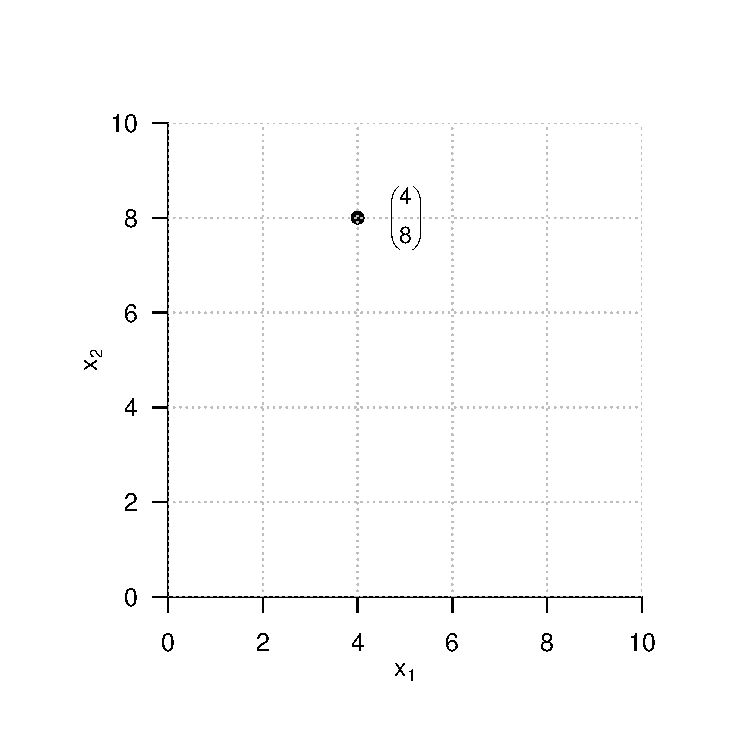
\includegraphics[width=0.4\linewidth]{0_2_Vektoren_files/figure-beamer/unnamed-chunk-6-1} 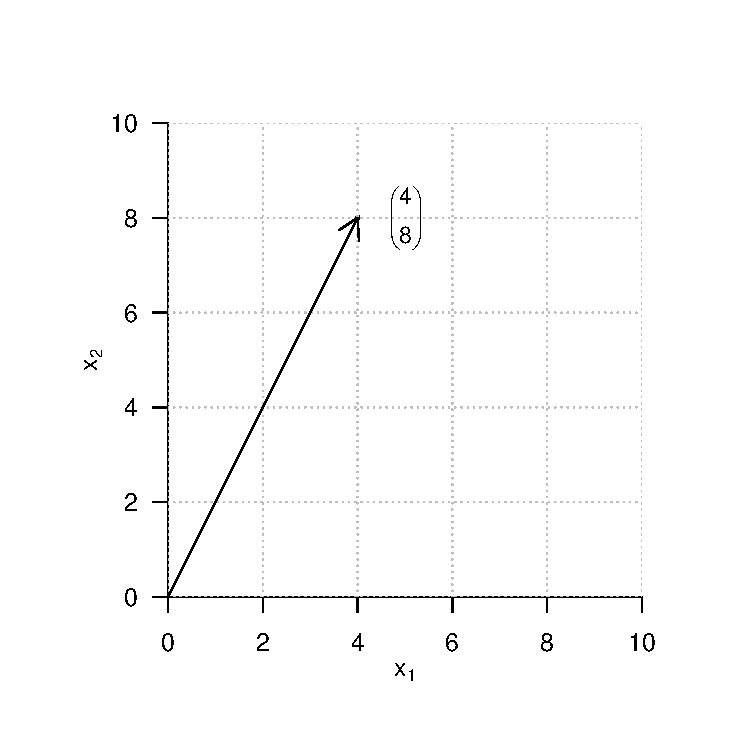
\includegraphics[width=0.4\linewidth]{0_2_Vektoren_files/figure-beamer/unnamed-chunk-6-2} \end{center}
\end{frame}

\begin{frame}{Reeller Vektorraum}
\protect\hypertarget{reeller-vektorraum-6}{}
\vspace{3mm}

\textcolor{darkcyan}{Vektoraddition in $\mathbb{R}^2$}

\vspace{9pt}
\small

\begin{align*}
\begin{pmatrix}
1 \\ 2
\end{pmatrix}
+
\begin{pmatrix}
3 \\ 1
\end{pmatrix}
=
\begin{pmatrix}
4 \\ 3
\end{pmatrix}
\end{align*}

\begin{center}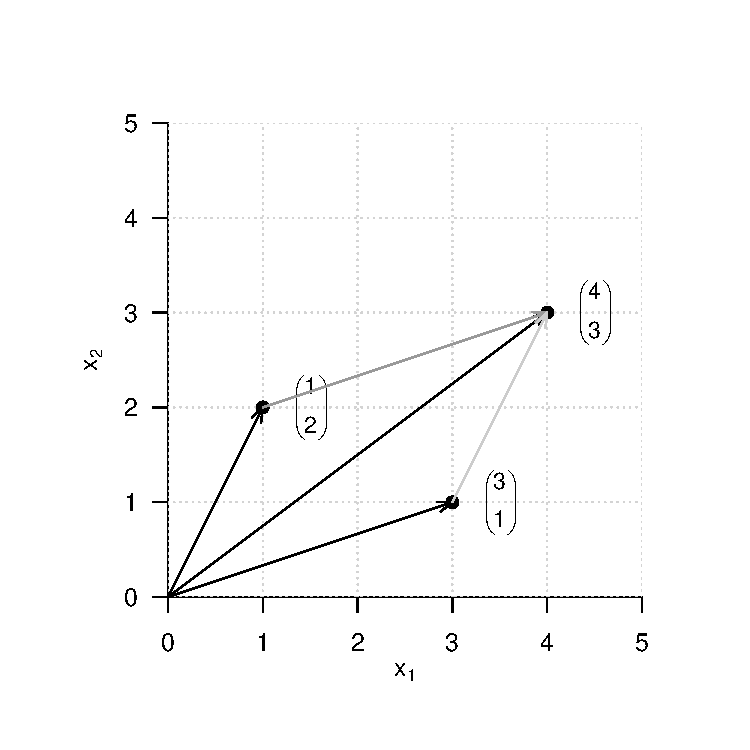
\includegraphics[width=0.4\linewidth]{0_2_Vektoren_files/figure-beamer/unnamed-chunk-7-1} \end{center}
\end{frame}

\begin{frame}{Reeller Vektorraum}
\protect\hypertarget{reeller-vektorraum-7}{}
\vspace{3mm}

\textcolor{darkcyan}{Vektorsubtraktion in $\mathbb{R}^2$}

\vspace{9pt}
\small

\begin{align*}
\begin{pmatrix}
1 \\ 2
\end{pmatrix}
-
\begin{pmatrix}
3 \\ 1
\end{pmatrix}
=
\begin{pmatrix}
1 \\ 2
\end{pmatrix}
+
\begin{pmatrix}
-3 \\ -1
\end{pmatrix}
=
\begin{pmatrix}
-2 \\ \,\, 1
\end{pmatrix}
\end{align*}

\begin{center}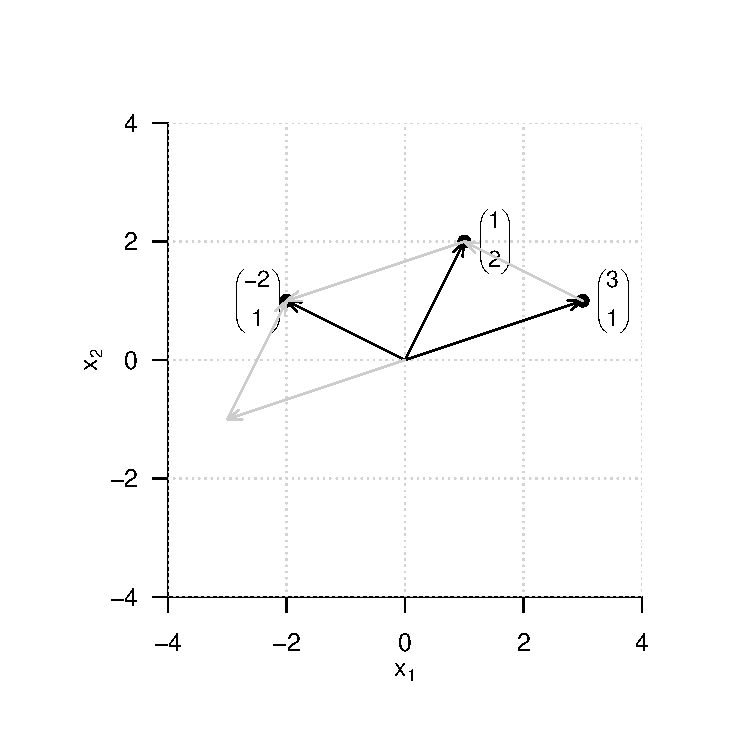
\includegraphics[width=0.4\linewidth]{0_2_Vektoren_files/figure-beamer/unnamed-chunk-8-1} \end{center}
\end{frame}

\begin{frame}{Reeller Vektorraum}
\protect\hypertarget{reeller-vektorraum-8}{}
\vspace{3mm}

\textcolor{darkcyan}{Skalarmultiplikation in $\mathbb{R}^2$}
\vspace{9pt} \small \begin{align*}
3
\begin{pmatrix}
1 \\ 1
\end{pmatrix}
=
\begin{pmatrix}
3 \\ 3
\end{pmatrix}
\end{align*}

\begin{center}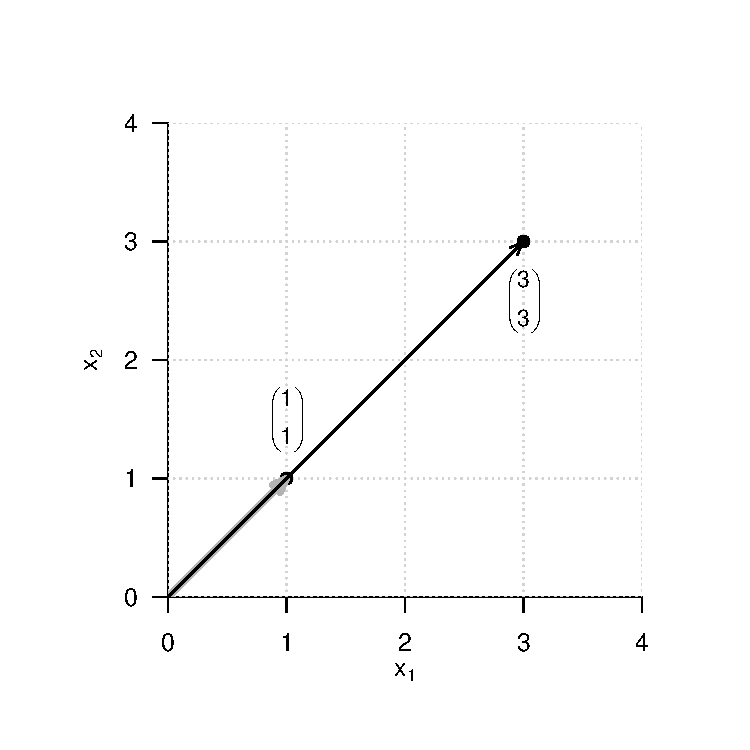
\includegraphics[width=0.4\linewidth]{0_2_Vektoren_files/figure-beamer/unnamed-chunk-9-1} \end{center}
\end{frame}

\begin{frame}{Vektoren}
\protect\hypertarget{vektoren-3}{}
\vspace{3mm}
\vfill
\setstretch{2.3}
\Large

Reeller Vektorraum

\textbf{Euklidischer Vektorraum}

Lineare Unabhängigkeit

Selbstkontrollfragen
\end{frame}

\begin{frame}{Euklidischer Vektorraum}
\protect\hypertarget{euklidischer-vektorraum}{}
\vspace{3mm}
\justifying
\setstretch{1.2}

\begin{definition}[Skalarprodukt auf $\mathbb{R}^m$]
\footnotesize
Das \textit{Skalarprodukt auf $\mathbb{R}^m$} ist definiert als die Abbildung
\begin{equation}
\langle \rangle : \mathbb{R}^m \times \mathbb{R}^m \to \mathbb{R}, (x,y) \mapsto \langle (x,y) \rangle := \langle x,y \rangle := \sum^m_{i=1}x_iy_i.
\end{equation}
\end{definition}

\small

Bemerkungen

\begin{itemize}
\tightlist
\item
  Das Skalarprodukt heißt Skalarprodukt, weil das Ergebnis ein Skalar
  ist, und nicht weil Skalare multipliziert werden.
\end{itemize}
\end{frame}

\begin{frame}[fragile]{Euklidischer Vektorraum}
\protect\hypertarget{euklidischer-vektorraum-1}{}
\vspace{3mm}

\textcolor{darkcyan}{Beispiel für Skalarprodukt}

\footnotesize

Es seien \begin{equation}
x:= \begin{pmatrix}1\\2\\3\end{pmatrix} \text{ und } y:= \begin{pmatrix}2\\0\\1\end{pmatrix}
\end{equation} Dann ergibt sich \begin{equation}
\langle x,y\rangle = x_1 y_1 + x_2 y_2 +  x_3  y_3 = 1 \cdot 2 + 2 \cdot 0 +  3 \cdot 1 = 2+0+3 = 5.
\end{equation}

\vspace{6pt}

\begin{Shaded}
\begin{Highlighting}[]
\CommentTok{\# Vektordefinition}
\NormalTok{x }\OtherTok{=} \FunctionTok{matrix}\NormalTok{(}\FunctionTok{c}\NormalTok{(}\DecValTok{1}\NormalTok{,}\DecValTok{2}\NormalTok{,}\DecValTok{3}\NormalTok{), }\AttributeTok{nrow =} \DecValTok{3}\NormalTok{)}
\NormalTok{y }\OtherTok{=} \FunctionTok{matrix}\NormalTok{(}\FunctionTok{c}\NormalTok{(}\DecValTok{2}\NormalTok{,}\DecValTok{0}\NormalTok{,}\DecValTok{1}\NormalTok{), }\AttributeTok{nrow =} \DecValTok{3}\NormalTok{)}
\end{Highlighting}
\end{Shaded}

\begin{Shaded}
\begin{Highlighting}[]
\CommentTok{\# Skalarprodukt mit R\textquotesingle{}s komponentenweiser Multiplikation (*) und sum()}
\FunctionTok{sum}\NormalTok{(x}\SpecialCharTok{*}\NormalTok{y)}
\end{Highlighting}
\end{Shaded}

\begin{verbatim}
> [1] 5
\end{verbatim}

\begin{Shaded}
\begin{Highlighting}[]
\CommentTok{\# Skalarprodukt mit R\textquotesingle{}s Matrixtransposition t() und {-}multiplikation (\%*\%)}
\FunctionTok{t}\NormalTok{(x) }\SpecialCharTok{\%*\%}\NormalTok{ y}
\end{Highlighting}
\end{Shaded}

\begin{verbatim}
>      [,1]
> [1,]    5
\end{verbatim}
\end{frame}

\begin{frame}{Euklidischer Vektorraum}
\protect\hypertarget{euklidischer-vektorraum-2}{}
\vspace{3mm}
\justify
\setstretch{1.2}

\begin{definition}[Euklidischer Vektorraum]
Das Tupel $((\mathbb{R}^m,+,\cdot),\langle\rangle)$ aus dem reellen Vektorraum $(\mathbb{R}^m,+,\cdot)$ und dem Skalarprodukt $\langle \rangle$ auf $\mathbb{R}^m$ heißt \textit{reeller kanonischer Euklidischer Vektorraum}.
\end{definition}

\small

Bemerkungen

\begin{itemize}
\tightlist
\item
  Generell heißt jedes Tupel aus einem Vektorraum (nicht nur reeller
  Vektorraum) und einem Skalarprodukt ``Euklidischer Vektorraum''.
\item
  Informell sprechen wir aber oft auch einfach von \(\mathbb{R}^m\) von
  ``Euklidischer Vektorraum'' und insbesondere bei
  \(((\mathbb{R}^m,+,\cdot),\langle\rangle)\) von ``Euklidischer
  Vektorraum''.
\item
  Der Unterschied zwischen einem Euklidischen Vektorraum und einem
  Vektorraum ist, dass es im Euklidischen Vektorraum neben
  Vektoraddition \((+)\) und Skalarmultiplikation \((\cdot)\) noch das
  Skalarprodukt \((\langle \rangle)\) gibt.
\item
  Ein Euklidischer Vektorraum ist ein Vektorraum mit geometrischer
  Struktur, die durch das Skalarprodukt induziert wird.
\item
  Mithilfe des Skalarproduktes können wir im Euklidischen Vektorraum die
  \emph{Länge} eines Vektors, den \emph{Abstand} zweier Vektoren und den
  \emph{Winkel} zwischen zwei Vektoren bestimmen.
\end{itemize}
\end{frame}

\begin{frame}{Euklidischer Vektorraum}
\protect\hypertarget{euklidischer-vektorraum-3}{}
\vspace{3mm}
\justify
\setstretch{1.2}
\small

\begin{definition}[Länge, Abstand, Winkel]
$((\mathbb{R}^m,+,\cdot),\langle\rangle)$ sei der Euklidische Vektorraum.
\begin{itemize}
\item Die \textit{Länge} eines Vektors $x \in \mathbb{R}^m$ ist definiert als
\begin{equation}
\lVert x \rVert := \sqrt{\langle x,x \rangle}.
\end{equation}
\item Der \textit{Abstand} zweier Vektoren $x,y \in \mathbb{R}^m$ ist definiert als
\begin{equation}
d(x,y) := \lVert x-y \rVert.
\end{equation}
\item Der \textit{Winkel} $\alpha$ zwischen zwei Vektoren $x,y \in \mathbb{R}^m$ mit $x,y \neq 0$ ist definiert durch \begin{equation}
0 \leq \alpha \leq \pi \text{ und } \cos\alpha := \frac{\langle x,y \rangle}{\lVert x \rVert\lVert y \rVert}
\end{equation}
\end{itemize}
\end{definition}

\footnotesize

Bemerkungen

\begin{itemize}
\item $\lVert x \rVert$ wird auch \textit{Norm von $x$} oder \textit{$\ell_2$-Norm von $x$} genannt.
\item Für den Abstand gilt, dass
\begin{itemize}
\footnotesize
\item $d(x,y) \geq 0$, $d(x,x) = 0$, $d(x,y) = d(y,x)$ und $d(x,y) \leq d(x,z) + d(z,y)$.
\end{itemize}
\item $\cos$ ist auf $[0, \pi]$ bijektiv, also invertierbar
\end{itemize}
\end{frame}

\begin{frame}{Euklidischer Vektorraum}
\protect\hypertarget{euklidischer-vektorraum-4}{}
\vspace{3mm}

\textcolor{darkcyan}{Beispiele für Vektorlängen in $\mathbb{R}^2$}
\vspace{9pt}

\begin{center}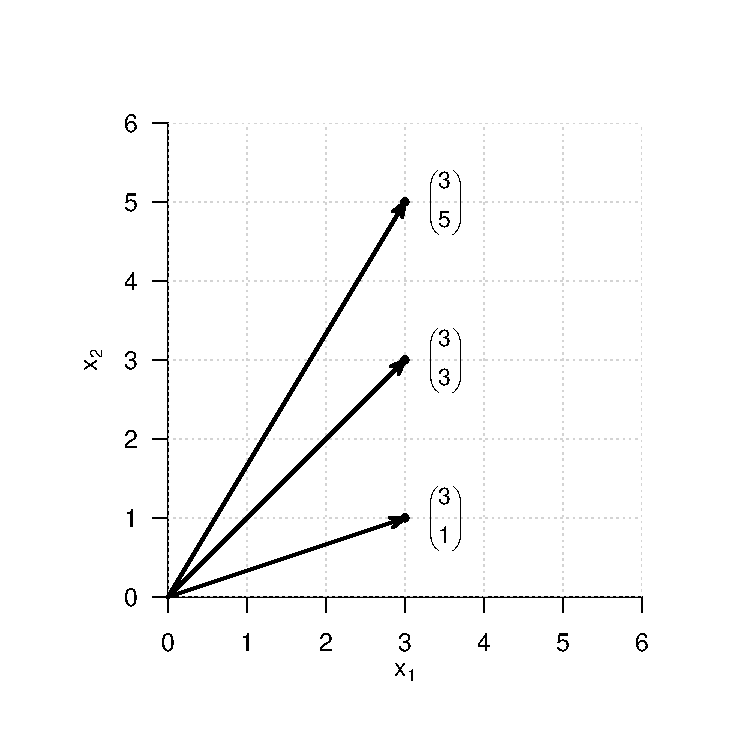
\includegraphics[width=0.5\linewidth]{0_2_Vektoren_files/figure-beamer/unnamed-chunk-15-1} \end{center}
\end{frame}

\begin{frame}[fragile]{Euklidischer Vektorraum}
\protect\hypertarget{euklidischer-vektorraum-5}{}
\vspace{3mm}

\textcolor{darkcyan}{Beispiele Vektorlängen in $\mathbb{R}^2$}

\footnotesize
\setstretch{1}

\begin{align*}
\left\lVert \begin{pmatrix}3\\5\end{pmatrix}\right\rVert = \sqrt{\left\langle \begin{pmatrix}3\\5\end{pmatrix} ,\begin{pmatrix}3\\5\end{pmatrix} \right\rangle} = \sqrt{3^2+5^2} = \sqrt{9+25} = \sqrt{34} \approx 5.83
\end{align*}

\begin{Shaded}
\begin{Highlighting}[]
\FunctionTok{norm}\NormalTok{(}\FunctionTok{matrix}\NormalTok{(}\FunctionTok{c}\NormalTok{(}\DecValTok{3}\NormalTok{,}\DecValTok{5}\NormalTok{), }\AttributeTok{nrow =} \DecValTok{2}\NormalTok{), }\AttributeTok{type =} \StringTok{"2"}\NormalTok{)  }\CommentTok{\# Vektorlänge = l\_2 Norm (type = "2")}
\end{Highlighting}
\end{Shaded}

\begin{verbatim}
> [1] 5.83
\end{verbatim}

\begin{align*}
\left\lVert \begin{pmatrix}3\\3\end{pmatrix}\right\rVert = \sqrt{\left\langle \begin{pmatrix}3\\3\end{pmatrix}, \begin{pmatrix}3\\3\end{pmatrix}\right\rangle} = \sqrt{3^2+3^2} = \sqrt{9+9} = \sqrt{18} \approx 4.24
\end{align*}

\begin{Shaded}
\begin{Highlighting}[]
\FunctionTok{norm}\NormalTok{(}\FunctionTok{matrix}\NormalTok{(}\FunctionTok{c}\NormalTok{(}\DecValTok{3}\NormalTok{,}\DecValTok{3}\NormalTok{), }\AttributeTok{nrow =} \DecValTok{2}\NormalTok{), }\AttributeTok{type =} \StringTok{"2"}\NormalTok{)  }\CommentTok{\# Vektorlänge = l\_2 Norm (type = "2")}
\end{Highlighting}
\end{Shaded}

\begin{verbatim}
> [1] 4.24
\end{verbatim}

\begin{align*}
\left\lVert \begin{pmatrix}3\\1\end{pmatrix}\right\rVert = \sqrt{\left\langle \begin{pmatrix}3\\1\end{pmatrix},\begin{pmatrix}3\\1\end{pmatrix} \right\rangle} = \sqrt{3^2+1^2} = \sqrt{9+1}
= \sqrt{10} \approx 3.16
\end{align*}

\begin{Shaded}
\begin{Highlighting}[]
\FunctionTok{norm}\NormalTok{(}\FunctionTok{matrix}\NormalTok{(}\FunctionTok{c}\NormalTok{(}\DecValTok{3}\NormalTok{,}\DecValTok{1}\NormalTok{), }\AttributeTok{nrow =} \DecValTok{2}\NormalTok{), }\AttributeTok{type =} \StringTok{"2"}\NormalTok{)  }\CommentTok{\# Vektorlänge = l\_2 Norm (type = "2")}
\end{Highlighting}
\end{Shaded}

\begin{verbatim}
> [1] 3.16
\end{verbatim}
\end{frame}

\begin{frame}{Euklidischer Vektorraum}
\protect\hypertarget{euklidischer-vektorraum-6}{}
\vspace{3mm}

\textcolor{darkcyan}{Beispiele für Abstände zwischen Vektoren in $\mathbb{R}^2$}
\vspace{9pt}

\begin{center}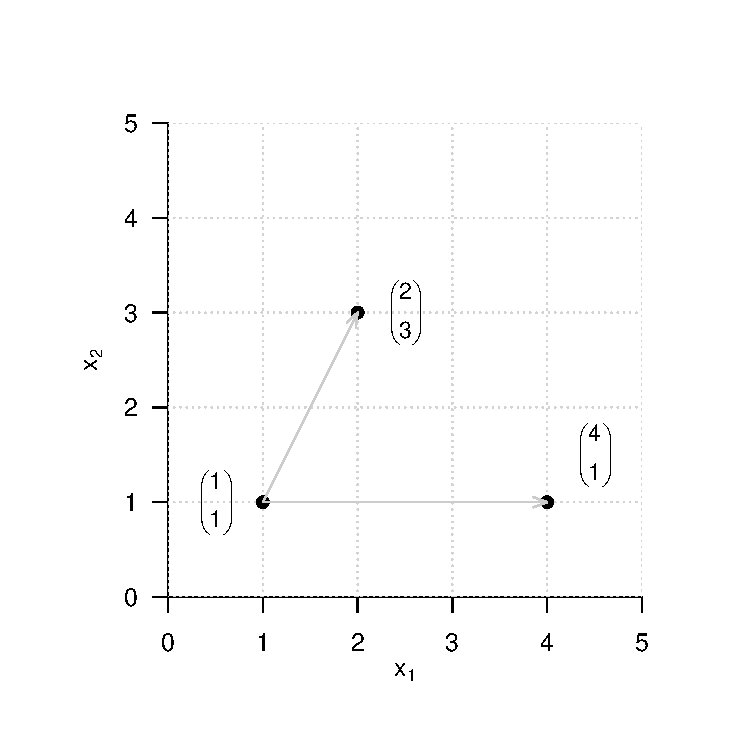
\includegraphics[width=0.5\linewidth]{0_2_Vektoren_files/figure-beamer/unnamed-chunk-19-1} \end{center}
\end{frame}

\begin{frame}[fragile]{Euklidischer Vektorraum}
\protect\hypertarget{euklidischer-vektorraum-7}{}
\vspace{3mm}

\textcolor{darkcyan}{Beispiele Abstände zwischen Vektoren in $\mathbb{R}^2$}
\footnotesize \setstretch{1}

\begin{align*}
d\left(\begin{pmatrix}1\\1\end{pmatrix}, \begin{pmatrix}2\\3\end{pmatrix}\right) = \left\lVert \begin{pmatrix}1\\1\end{pmatrix} - \begin{pmatrix}2\\3\end{pmatrix}\right\rVert = \left\lVert \begin{pmatrix}-1\\-2\end{pmatrix}\right\rVert = \sqrt{(-1)^2+(-2)^2} = \sqrt{5} \approx 2.24
\end{align*}

\begin{Shaded}
\begin{Highlighting}[]
\FunctionTok{norm}\NormalTok{(}\FunctionTok{matrix}\NormalTok{(}\FunctionTok{c}\NormalTok{(}\DecValTok{1}\NormalTok{,}\DecValTok{1}\NormalTok{), }\AttributeTok{nrow =} \DecValTok{2}\NormalTok{) }\SpecialCharTok{{-}} \FunctionTok{matrix}\NormalTok{(}\FunctionTok{c}\NormalTok{(}\DecValTok{2}\NormalTok{,}\DecValTok{3}\NormalTok{), }\AttributeTok{nrow =} \DecValTok{2}\NormalTok{), }\AttributeTok{type =} \StringTok{"2"}\NormalTok{)}
\end{Highlighting}
\end{Shaded}

\begin{verbatim}
> [1] 2.24
\end{verbatim}

\begin{align*}
d\left(\begin{pmatrix}1\\1\end{pmatrix}, \begin{pmatrix}4\\1\end{pmatrix}\right) = \left\lVert \begin{pmatrix}1\\1\end{pmatrix} - \begin{pmatrix}4\\1\end{pmatrix}\right\rVert = \left\lVert \begin{pmatrix}-3\\0\end{pmatrix}\right\rVert = \sqrt{(-3)^2+0^2} = \sqrt{9} = 3
\end{align*}

\begin{Shaded}
\begin{Highlighting}[]
\FunctionTok{norm}\NormalTok{(}\FunctionTok{matrix}\NormalTok{(}\FunctionTok{c}\NormalTok{(}\DecValTok{1}\NormalTok{,}\DecValTok{1}\NormalTok{), }\AttributeTok{nrow =} \DecValTok{2}\NormalTok{) }\SpecialCharTok{{-}} \FunctionTok{matrix}\NormalTok{(}\FunctionTok{c}\NormalTok{(}\DecValTok{4}\NormalTok{,}\DecValTok{1}\NormalTok{), }\AttributeTok{nrow =} \DecValTok{2}\NormalTok{), }\AttributeTok{type =} \StringTok{"2"}\NormalTok{)}
\end{Highlighting}
\end{Shaded}

\begin{verbatim}
> [1] 3
\end{verbatim}
\end{frame}

\begin{frame}{Euklidischer Vektorraum}
\protect\hypertarget{euklidischer-vektorraum-8}{}
\vspace{3mm}

Kosinus und Arkuskosinus auf \([0,\pi]\) \setstretch{1} \vspace{6pt}

\begin{center}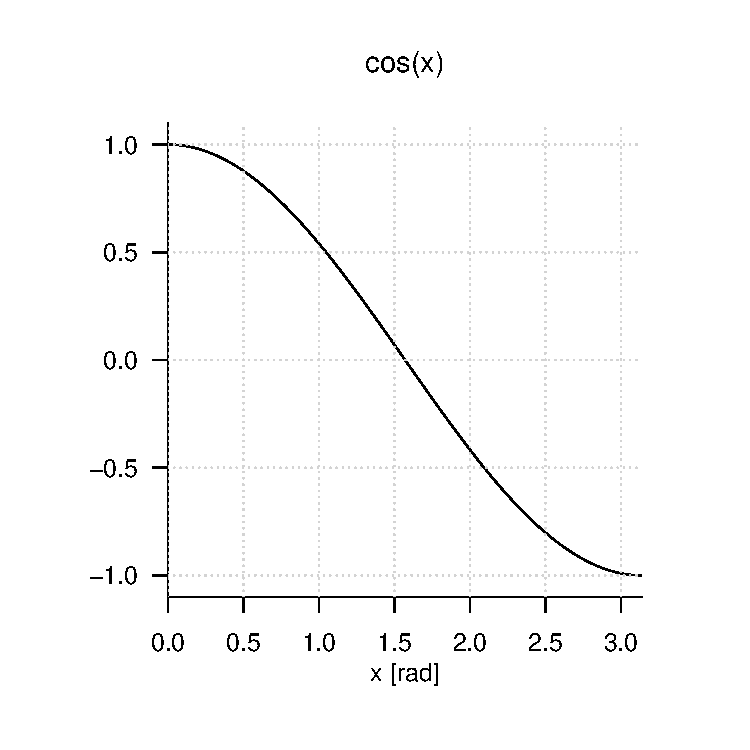
\includegraphics[width=0.35\linewidth]{0_2_Vektoren_files/figure-beamer/unnamed-chunk-22-1} 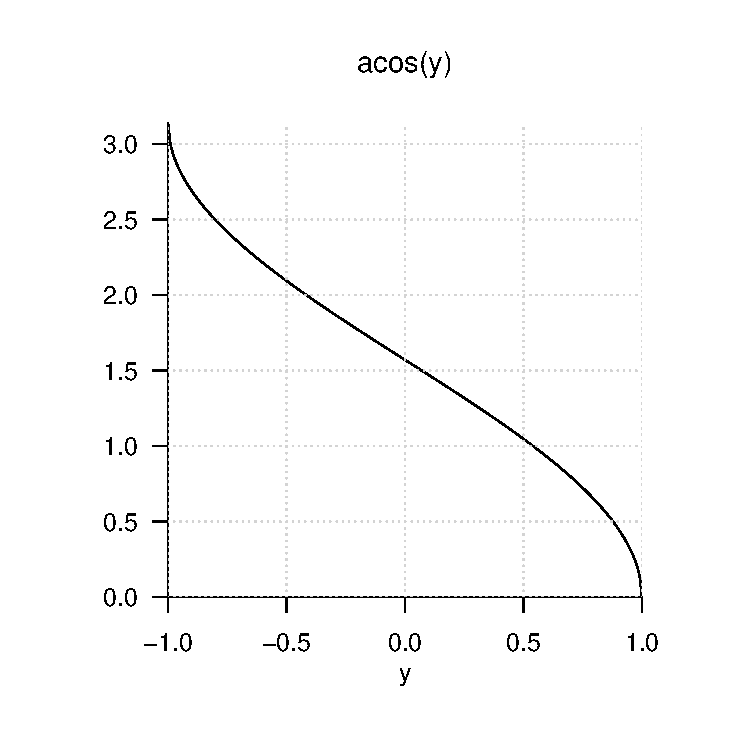
\includegraphics[width=0.35\linewidth]{0_2_Vektoren_files/figure-beamer/unnamed-chunk-22-2} \end{center}
\small
\vspace{5pt}

Umrechnung zwischen Gradmaß {[}deg{]} und Bogenmaß {[}rad{]}:
\vspace{3pt} \footnotesize \begin{equation}
\mbox{deg} = \mbox{rad} \cdot \frac{180}{\pi}, \,
\mbox{rad} = \mbox{deg} \cdot \frac{\pi}{180}
\end{equation}

\small

\textcolor{darkcyan}{Beispiele} \footnotesize \begin{align*}
0\pi \mbox{ rad }                 = 0.00 \mbox{ rad } = 0  \mbox{ deg }, \,
\frac{\pi}{2} \mbox{ rad } \approx  1.57 \mbox{ rad } = 90 \mbox{ deg }, \,
\pi \mbox{ rad } \approx  3.14 \mbox{ rad } = 180 \mbox{ deg }
\end{align*}
\end{frame}

\begin{frame}{Euklidischer Vektorraum}
\protect\hypertarget{euklidischer-vektorraum-9}{}
\vspace{3mm}

\textcolor{darkcyan}{Beispiele für Winkel zwischen Vektoren in $\mathbb{R}^2$}

\vspace{6pt}

\begin{center}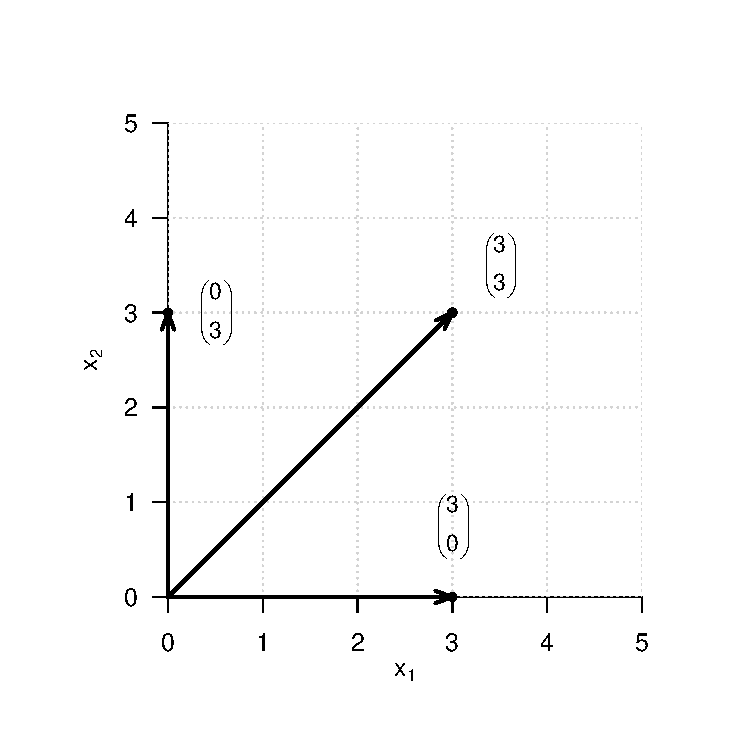
\includegraphics[width=0.5\linewidth]{0_2_Vektoren_files/figure-beamer/unnamed-chunk-23-1} \end{center}
\end{frame}

\begin{frame}[fragile]{Euklidischer Vektorraum}
\protect\hypertarget{euklidischer-vektorraum-10}{}
\vspace{3mm}

\textcolor{darkcyan}{Beispiel 1) für Winkel zwischen Vektoren in $\mathbb{R}^2$}

\vspace{6pt}
\small

Winkel in Radians

\footnotesize

\begin{align*}
\alpha = \mbox{acos} \left ( \frac{\left \langle \begin{pmatrix} 3\\0 \end{pmatrix}, \begin{pmatrix} 3\\3 \end{pmatrix} \right \rangle}{\left \lVert \begin{pmatrix}3\\0\end{pmatrix}\right \rVert\left \lVert \begin{pmatrix}3\\3\end{pmatrix}\right \rVert}\right)
= \mbox{acos}\left(\frac{3 \cdot 3 + 0 \cdot 3}{\sqrt{3^2 + 0^2} \cdot \sqrt{3^2 + 3^2}}\right)
= \mbox{acos}\left(\frac{9}{3 \cdot \sqrt{18}}\right)
= \frac{\pi}{4} \approx 0.785
\end{align*}

\vspace{6pt}
\small

Winkel in Grad

\footnotesize

\begin{align*}
\frac{\pi}{4} \cdot \frac{180}{\pi} = 45
\end{align*}

\small

Berechnung in R \footnotesize

\begin{Shaded}
\begin{Highlighting}[]
\NormalTok{x }\OtherTok{=} \FunctionTok{matrix}\NormalTok{(}\FunctionTok{c}\NormalTok{(}\DecValTok{3}\NormalTok{,}\DecValTok{0}\NormalTok{), }\AttributeTok{nrow =} \DecValTok{2}\NormalTok{)                                   }\CommentTok{\# Vektor 1}
\NormalTok{y }\OtherTok{=} \FunctionTok{matrix}\NormalTok{(}\FunctionTok{c}\NormalTok{(}\DecValTok{3}\NormalTok{,}\DecValTok{3}\NormalTok{), }\AttributeTok{nrow =} \DecValTok{2}\NormalTok{)                                   }\CommentTok{\# Vektor 2}
\NormalTok{w }\OtherTok{=} \FunctionTok{acos}\NormalTok{(}\FunctionTok{sum}\NormalTok{(x}\SpecialCharTok{*}\NormalTok{y)}\SpecialCharTok{/}\NormalTok{(}\FunctionTok{sqrt}\NormalTok{(}\FunctionTok{sum}\NormalTok{(x}\SpecialCharTok{*}\NormalTok{x))}\SpecialCharTok{*}\FunctionTok{sqrt}\NormalTok{(}\FunctionTok{sum}\NormalTok{(y}\SpecialCharTok{*}\NormalTok{y)))) }\SpecialCharTok{*} \DecValTok{180}\SpecialCharTok{/}\NormalTok{pi    }\CommentTok{\# Winkel in Grad}
\FunctionTok{print}\NormalTok{(w)}
\end{Highlighting}
\end{Shaded}

\begin{verbatim}
> [1] 45
\end{verbatim}
\end{frame}

\begin{frame}[fragile]{Euklidischer Vektorraum}
\protect\hypertarget{euklidischer-vektorraum-11}{}
\vspace{3mm}

\textcolor{darkcyan}{Beispiel 2) für Winkel zwischen Vektoren in $\mathbb{R}^2$}

\vspace{6pt}
\small

Winkel in Radians

\footnotesize

\begin{align*}
\alpha = \mbox{acos}  \left ( \frac{\left \langle \begin{pmatrix} 3\\0 \end{pmatrix}, \begin{pmatrix} 0\\3 \end{pmatrix} \right \rangle}{\left \lVert \begin{pmatrix}3\\0\end{pmatrix}\right \rVert \left \lVert\begin{pmatrix}0\\3\end{pmatrix}\right \rVert}\right)
= \mbox{acos}\left(\frac{3 \cdot 0 + 0 \cdot 3}{\sqrt{3^2 + 0^2} \cdot \sqrt{0^2 + 3^2}}\right)
= \mbox{acos}\left(\frac{0}{3 \cdot \sqrt{3\cdot 3}}\right)
= \frac{\pi}{2} \approx 1.57
\end{align*}

\vspace{6pt}
\small

Winkel in Grad

\footnotesize

\begin{align*}
\frac{\pi}{2} \cdot \frac{180}{\pi} = 90
\end{align*}

\small

Berechnung in R \footnotesize

\begin{Shaded}
\begin{Highlighting}[]
\NormalTok{x }\OtherTok{=} \FunctionTok{matrix}\NormalTok{(}\FunctionTok{c}\NormalTok{(}\DecValTok{3}\NormalTok{,}\DecValTok{0}\NormalTok{), }\AttributeTok{nrow =} \DecValTok{2}\NormalTok{)                                   }\CommentTok{\# Vektor 1}
\NormalTok{y }\OtherTok{=} \FunctionTok{matrix}\NormalTok{(}\FunctionTok{c}\NormalTok{(}\DecValTok{0}\NormalTok{,}\DecValTok{3}\NormalTok{), }\AttributeTok{nrow =} \DecValTok{2}\NormalTok{)                                   }\CommentTok{\# Vektor 2}
\NormalTok{w }\OtherTok{=} \FunctionTok{acos}\NormalTok{(}\FunctionTok{sum}\NormalTok{(x}\SpecialCharTok{*}\NormalTok{y)}\SpecialCharTok{/}\NormalTok{(}\FunctionTok{sqrt}\NormalTok{(}\FunctionTok{sum}\NormalTok{(x}\SpecialCharTok{*}\NormalTok{x))}\SpecialCharTok{*}\FunctionTok{sqrt}\NormalTok{(}\FunctionTok{sum}\NormalTok{(y}\SpecialCharTok{*}\NormalTok{y)))) }\SpecialCharTok{*} \DecValTok{180}\SpecialCharTok{/}\NormalTok{pi    }\CommentTok{\# Winkel in Grad}
\FunctionTok{print}\NormalTok{(w)}
\end{Highlighting}
\end{Shaded}

\begin{verbatim}
> [1] 90
\end{verbatim}
\end{frame}

\begin{frame}{Euklidischer Vektorraum}
\protect\hypertarget{euklidischer-vektorraum-12}{}
\vspace{3mm}
\setstretch{1.2}
\small
\begin{definition}[Orthogonalität und Orthonormalität von Vektoren]
\justifying
$\left((\mathbb{R}^m, +, \cdot), \langle \rangle \right)$ sei der Euklidische Vektorraum.
\begin{itemize}
\item Zwei Vektoren $x,y \in \mathbb{R}^m$ heißen \textit{orthogonal}, wenn gilt, dass
\begin{equation}
\langle x, y \rangle = 0
\end{equation}
\item Zwei Vektoren $x,y \in \mathbb{R}^m$ heißen \textit{orthonormal}, wenn gilt, dass
\begin{equation}
\langle x, y \rangle = 0 \mbox{ und } \Vert x \Vert = \Vert y \Vert = 1.
\end{equation}
\end{itemize}
\end{definition}

Bemerkungen

\begin{itemize}
\tightlist
\item
  Für orthogonale und orthonormale Vektoren gilt insbesondere auch
\end{itemize}

\begin{equation}
\cos \alpha
= \frac{\langle x, y \rangle}{\Vert x \Vert \Vert y \Vert}
= \frac{0}{\Vert x \Vert \Vert y \Vert}
= 0
\end{equation} also \begin{equation}
\alpha = \frac{\pi}{2} = 90^{\circ}
\end{equation}
\end{frame}

\begin{frame}{Vektoren}
\protect\hypertarget{vektoren-4}{}
\vspace{3mm}
\vfill
\setstretch{2.3}
\Large

Reeller Vektorraum

Euklidischer Vektorraum

\textbf{Lineare Unabhängigkeit}

Selbstkontrollfragen
\end{frame}

\begin{frame}{Lineare Unabhängigkeit}
\protect\hypertarget{lineare-unabhuxe4ngigkeit}{}
\vspace{3mm}
\setstretch{1}
\small
\begin{definition}[Linearkombination]
\justifying
$\{v_1, v_2, ..., v_k\}$ sei eine Menge von $k$ Vektoren eines Vektorraums $V$.
Dann ist die \textit{Linearkombination} der Vektoren in $v_1, v_2, ..., v_k$ mit den
skalaren Koeffizienten $a_1, a_2,...,a_k$ definiert als der Vektor
\begin{equation}
w := \sum_{i=1}^k a_i v_i \in V.
\end{equation}
\end{definition}

\textcolor{darkcyan}{Beispiel einer Linearkombination}

\footnotesize

Es seien \begin{align*}
v_1 := \begin{pmatrix} 2 \\ 1 \end{pmatrix},
v_2 := \begin{pmatrix} 1 \\ 1 \end{pmatrix},
v_3 := \begin{pmatrix} 0 \\ 1 \end{pmatrix}
\mbox{ und }
a_1 := 2, a_2 := 3, a_3 := 0.
\end{align*} Dann ergibt sich \begin{align*}
\begin{split}
w
  = a_1v_1 + a_2v_2 + a_3v_3
& =  2 \cdot \begin{pmatrix} 2 \\ 1 \end{pmatrix}
   + 3 \cdot \begin{pmatrix} 1 \\ 1 \end{pmatrix}
   + 0 \cdot \begin{pmatrix} 0 \\ 1 \end{pmatrix}   \\
& =   \begin{pmatrix} 4 \\ 2 \end{pmatrix}
    + \begin{pmatrix} 3 \\ 3 \end{pmatrix}
    + \begin{pmatrix} 0 \\ 0 \end{pmatrix}   \\
& =   \begin{pmatrix} 7 \\ 5 \end{pmatrix}
\end{split}
\end{align*}
\end{frame}

\begin{frame}{Lineare Unabhängigkeit}
\protect\hypertarget{lineare-unabhuxe4ngigkeit-1}{}
\vspace{3mm}
\small
\begin{definition}[Lineare Unabhängigkeit]
\justifying
$V$ sei ein Vektorraum. Eine Menge $W := \{w_1, w_2, ...,w_k\}$ von Vektoren in $V$ heißt
\textit{linear unabhängig}, wenn die einzige Repräsentation des Nullelements
$0 \in V$ durch eine Linearkombination der $w \in W$ die triviale
Repräsentation
\begin{equation}
0 = a_1 w_1 + a_2 w_2 + \cdots + a_k w_k \mbox{ mit } a_1 = a_2 =  \cdots = a_k = 0
\end{equation}
ist. Wenn die Menge $W$ nicht linear unabhängig ist, dann heißt sie \textit{linear abhängig}.
\end{definition}

Bemerkungen

\begin{itemize}
\tightlist
\item
  Prinzipiell müsste man für jede Linearkombination der \(w \in W\)
  prüfen, ob sie Null ist.
\item
  Die beiden folgenden Theoreme zeigen, dass es auch einfacher geht.
\end{itemize}
\end{frame}

\begin{frame}{Lineare Unabhängigkeit}
\protect\hypertarget{lineare-unabhuxe4ngigkeit-2}{}
\vspace{3mm}
\small
\begin{theorem}[Lineare Abhängigkeit von zwei Vektoren]
\justifying
\normalfont
$V$ sei ein Vektorraum. Zwei Vektoren $v_1, v_2 \in V$ sind linear abhängig,
wenn einer der Vektoren ein skalares Vielfaches des anderen Vektors ist.
\end{theorem}

\footnotesize

\underline{Beweis} \vspace{1mm} \(v_1\) sei ein skalares Vielfaches von
\(v_2\), also \begin{equation}
v_1 = \lambda v_2 \mbox{ mit } \lambda \neq 0.
\end{equation} Dann gilt \begin{equation}
v_1 - \lambda v_2 = 0.
\end{equation} Dies wiederum entspricht der Linearkombination
\begin{equation}
a_1v_1 + a_2v_2 = 0
\end{equation} mit \(a_1 = 1 \neq 0\) und \(a_2 = -\lambda \neq 0\). Es
gibt also eine Linearkombination des Nullelementes, die nicht die
triviale Repräsentation ist, und damit sind \(v_1\) und \(v_2\) nicht
linear unabhängig.
\end{frame}

\begin{frame}{Lineare Unabhängigkeit}
\protect\hypertarget{lineare-unabhuxe4ngigkeit-3}{}
\vspace{3mm}
\small

\textcolor{darkcyan}{Beispiel linear abhängiger Vektoren}

\footnotesize

Es seien \begin{align*}
v_1 = \begin{pmatrix} 3 \\ 3 \end{pmatrix} \text{ und }
v_2 = \begin{pmatrix} 1 \\ 1 \end{pmatrix}.
\end{align*} \(v_1\) ist also ein skalares Vielfaches von \(v_2\), also
\begin{equation}
v_1 = \lambda v_2 \mbox{ mit } \lambda =3.
\end{equation} Dann gilt

\begin{equation}
v_1 - \lambda v_2 = \begin{pmatrix} 3 \\ 3 \end{pmatrix} -
\lambda \begin{pmatrix} 1 \\ 1 \end{pmatrix} = 0.
\end{equation}

Dies wiederum entspricht der Linearkombination \begin{equation}
a_1v_1 + a_2v_2 = 0
\end{equation} mit \(a_1 = 1 \neq 0\) und \(a_2 = -\lambda \neq 0\).
\end{frame}

\begin{frame}{Lineare Unabhängigkeit}
\protect\hypertarget{lineare-unabhuxe4ngigkeit-4}{}
\vspace{3mm}
\setstretch{1.1}
\small
\begin{theorem}[Lineare Abhängigkeit einer Menge von Vektoren]
\justifying
\normalfont
$V$ sei ein Vektorraum und $w_1,...,w_k \in V$ sei eine Menge von Vektoren in $V$.
Wenn einer der Vektoren $w_i, i = 1,...,k$ eine Linearkombination der anderen
Vektoren ist, dann ist die Menge der Vektoren linear abhängig.
\end{theorem}

\footnotesize

\underline{Beweis}

Die Vektoren \(w_1,...,w_k\) sind genau dann linear abhängig, wenn gilt,
dass \(\sum_{i=1}^n a_i w_i = 0\) mit mindestens einem \(a_i \neq 0\) .
Es sei also zum Beispiel \(a_j \neq 0\). Dann gilt \begin{equation}
0 = \sum_{i=1}^n a_i w_i = \sum_{i=1, i \neq j}^n a_i w_i + a_jw_j
\end{equation} Also folgt \begin{equation}
a_jw_j  = - \sum_{i=1, i \neq j}^n a_i w_i
\end{equation} und damit \begin{equation}
w_j  = - a_j^{-1}\sum_{i=1, i \neq j}^n a_i w_i = - \sum_{i=1, i \neq j}^n (a_j^{-1}a_i) w_i
\end{equation} Also ist \(w_j\) eine Linearkombination der
\(w_i, i = 1,...,k\) mit \(i \neq j\). \(\hfill \Box\)
\end{frame}

\begin{frame}{Vektoren}
\protect\hypertarget{vektoren-5}{}
\vfill
\setstretch{2.3}
\Large

Reeller Vektorraum

Euklidischer Vektorraum

Lineare Unabhängigkeit

\textbf{Selbstkontrollfragen}
\end{frame}

\begin{frame}{Selbstkontrollfragen}
\protect\hypertarget{selbstkontrollfragen}{}
\footnotesize
\setstretch{1.5}

\begin{enumerate}
\tightlist
\item
  Geben Sie die Definition eines Vektorraums wieder.
\item
  Geben Sie die Definition des reellen Vektorraums wieder.
\item
  Es seien \begin{equation}
  x := \begin{pmatrix} 2 \\ 1 \end{pmatrix}, 
  y := \begin{pmatrix} 0 \\ 1 \end{pmatrix}
  \mbox{ und } 
  a := 2. 
  \end{equation} Berechnen Sie \begin{equation}
  v = a(x+y) \mbox{ und } w = \frac{1}{a}(y-x)
  \end{equation} und überprüfen Sie ihre Rechnung mit R.
\item
  Geben Sie die Definition des Skalarproduktes auf \(\mathbb{R}^m\)
  wieder.
\item
  Für \begin{equation}
  x := \begin{pmatrix} 2 \\ 1 \\ 3 \end{pmatrix},
  y := \begin{pmatrix} 1 \\ 0 \\ 1 \end{pmatrix},
  z := \begin{pmatrix} 3 \\ 1 \\ 0 \end{pmatrix} 
  \end{equation} berechnen Sie \begin{equation}
  \langle x,y \rangle, \langle x, z \rangle, \langle y,z \rangle
  \end{equation} und überprüfen Sie ihre Rechnung mithilfe von R.
\item
  Geben Sie die Definition des Euklidischen Vektorraums wieder.
\item
  Definieren Sie die Länge eines Vektors im Euklidischen Vektorraum.
\item
  Berechnen Sie die Längen der Vektoren \(x,y,z\) aus Aufgabe 5 und
  überprüfen Sie ihre Rechnung mit R.
\end{enumerate}
\end{frame}

\begin{frame}{Selbstkontrollfragen}
\protect\hypertarget{selbstkontrollfragen-1}{}
\footnotesize
\setstretch{1.9}

\begin{enumerate}
\setcounter{enumi}{8}
\tightlist
\item
  Geben Sie Definition des Abstands zweier Vektoren im Euklidischen
  Vektorraum wieder.
\item
  Berechnen Sie \(d(x,y), d(x,z)\) und \(d(y,z)\) für \(x,y,z\) aus
  Aufgabe 5.
\item
  Geben Sie die Definition des Winkels zwischen zwei Vektoren im
  Euklidischen Vektorraum wieder.
\item
  Berechnen Sie die Winkel zwischen den Vektoren \(x\) und \(y\), \(x\)
  und \(z\), sowie \(y\) und \(z\) aus Aufgabe 5 mit R.
\item
  Definieren Sie die Begriffe der Orthogonalität und Orthonormalität von
  Vektoren.
\item
  Definieren Sie den Begriff der Linearkombination von Vektoren.
\item
  Definieren Sie den Begriff der linearen Unabhängigkeit von Vektoren.
\item
  Woran kann man erkennen, dass zwei Vektoren linear abhängig sind?
\item
  Dokumentieren Sie alle in dieser Einheit eingeführten R Befehle in
  einem Skript.
\end{enumerate}
\end{frame}

\end{document}
